%----------------------------------
\chapter{Product Specification}\hyperdef{part}{spec}{}\label{ch:spec}
%----------------------------------

\section{Conceptual Design}

The \ModelDesc addresses the
problems of building the heavenly body basis of the JEOD reference frame tree
and of representing the translational and rotational states of those heavenly
bodies. This section describes the conceptual design of the model.
The first subsection describes concepts that are critical in understanding
the model. The second subsection describes the modules that form the model.


\subsection{Key Concepts}
\subsubsection{Reference Frames and the Reference Frame Tree}
The JEOD concept of a reference frame is the centralizing feature of JEOD.
Planets contain reference frames, vehicles contain reference frames,
and various derived frames augment these planetary and vehicular frames.
Reference frames contain state and connectivity information.
The state aspect of a reference frame provides the means to represent the
translational and rotational states of the entity associated with the
reference frame.
The connectivity aspect of a reference frame provides the means to connect one
reference frame to another, eventually forming the JEOD reference frame tree.
All active reference frames are a part of this reference frame tree.

The \ModelDesc plays a key role in forming the basis of the reference frame tree
and in populating the states of those frames that represent heavenly bodies.
The root of the reference frame tree is the one true inertial
reference frame of a simulation. (This assumes the existence of a Newtonian
inertial reference frame. There is no such thing, but the errors are negligibly
small with the appropriate choice.) This root frame is always established by
some ephemeris model. The frames representing the Sun and the planets descend
from this root frame. The connectivities between these heavenly body frames
and the states of these frames are also established by some ephemeris model.

The ephemeris models must construct the heavenly body portion of the
JEOD reference frame tree in a way that is consistent with how the
\GRAVITY\ computes gravitation. That model calculates gravitational acceleration
per Newton's law of gravitation for gravitating bodies that are at or below a
vehicle's integration frame, but calculated it as a third body effect otherwise.

\subsubsection{Ephemeris Model}
As used in JEOD, an ephemeris model is a model that provides
a means for determining the translational and/or rotational
states of heavenly bodies as a function of time. Multiple JEOD models
make use of various ephemerides. Ephemerides are essential
in propagating the state of a vehicle that is gravitationally attracted
to multiple heavenly bodies. The need for ephemeris models in JEOD
goes much deeper than this. An ephemeris model of some sort is needed
in almost every JEOD-based simulation. All vehicle-based reference frames
are represented with respect to some parent ephemeris-based
reference frame.

\subsubsection{JPL Development Ephemeris Models}
The Russian Institute for Applied Astronomy, the Paris Observatory,
and the Jet Propulsion Laboratory (JPL) are the three leading institutions
that provide high precision ephemerides of solar system bodies.
JEOD uses the JPL Development Ephemeris (DE) models. Three such models are
provided with JEOD, the DE405, DE421 and DE440 models.

\subsubsection{Ephemeris Item}
A JEOD ephemeris model represents the translational and/or rotational
states of one or more heavenly bodies as a function of time.
Note the \REFFRAMES\ already provides the standard mechanism in JEOD
for representing such states.
An issue can arise with the use of multiple ephemeris models:
What if multiple ephemeris models provide potentially conflicting
representations of the same quantity?
The solution to this problem is to provide a bridge between the
ephemeris models and the states they can provide.
The ephemeris items are the abstract representation of this bridge.

\subsubsection{Ephemeris Manager}
The ephemeris models collectively form the basis of the JEOD reference
frame tree. Something is needed to ride herd over the ephemeris models
to make this happen. This `something' is the ephemeris manager.

\subsubsection{Subscription}
Computing planetary ephemerides would pose an unnecessary computational expense
were all possible heavenly bodies represented in every JEOD-based simulation.
To avoid this problem, the reference frame tree is constructed and states
are computed only for those bodies needed elsewhere in the simulation.
This need is assessed based on the reference frame subscription model.
Models that need to use some aspect of a reference frame register a
subscription to that frame. The \ModelDesc components build the heavenly
body basis of the reference frame tree based upon these subscriptions.
Only those items that are needed are placed in the active reference frame tree.


\subsection{Model Components}
The \ModelDesc comprises a set of modules that address different aspects of the
problems that need to be solved by the model.
Each such module is a separate subdirectory of the root
model directory, \verb|$JEOD_HOME/models/environment/ephemerides|.
\subsubsection{Ephemeris Item}
The ephemeris item module (model subdirectory ephem\_item)
implements the concept of an ephemeris item.
The class \texttt{EphemerisItem} establishes the abstract basis of this concept.
The derived class \texttt{EphemerisPoint} pertains to translational states
while \texttt{EphemerisOrientation} pertains to rotational states.
A specialization of the \texttt{EphemerisOrientation} class,
\texttt{EphemerisZXZOrientation}, pertains to ephemeris models that represent
orientation in terms of a classical (z-x-z) Euler sequence.
Figure~\ref{fig:ephem_item_classes} depicts the ephemeris items
defined in the \ModelDesc.
\begin{figure}[hbtp]
\centering
\includegraphics{ephem_item}
\caption{Ephemeris Items and Ephemeris Reference Frames}
\label{fig:ephem_item_classes}
\end{figure}

\subsubsection{Ephemeris Interface}
The ephemeris interface module (model subdirectory ephem\_interface)
defines several classes.\begin{description}
\item[Ephemerides Model Messages] The class \texttt{EphemeridesMessages} is a
standard message identifier class. It defines the message identifiers for all
of the messages generated by the \ModelDesc.
\item[Ephemeris Reference Frame] The class \texttt{EphemerisRefFrame}
(depicted in figure~\ref{fig:ephem_item_classes}), derives from the
\texttt{RefFrame} class. 
\begin{figure}[hbtp]
\centering
\includegraphics{ephem_interface}
\caption{Ephemeris Interface}
\label{fig:ephem_interface_classes}
\end{figure}
\item[Ephemeris Interface] The class \texttt{EphemerisInterface} defines,
in an abstract sense, the basic characteristics of an ephemeris model.
All JEOD ephemeris models are an instances of some class that derives from
\texttt{EphemerisInterface}.
An ephemeris model will be called upon to build its share of the reference frame
tree via a prescribed sequence of actions. The model will also be called
to update the ephemeris items for which it is responsible.
The former happen at initialization time and whenever the reference tree might
change due to subscription changes; the updates are performed on a
scheduled basis.
Figure~\ref{fig:ephem_interface_classes} depicts the ephemeris models
defined in the \ModelDesc.
\item[Single Point Ephemeris] Very simple simulations only need a very simple
ephemeris model, one that describes the sole inertial frame in the
simulation. The class \texttt{SinglePointEphemeris}
provides a simple model where there is but one EphemerisPoint in the entire
simulation.
\item[Empty Space Ephemeris] The simplest of all simulations
involves vehicles operating in otherwise empty space.
The class \texttt{EmptySpaceEphemeris}
specializes the class \texttt{SinglePointEphemeris} for use in
simulations that does not involve any gravitating bodies: Empty space.
The root node of the reference frame tree
is the one and only ephemeris reference frame in the simulation.
\item[Single Planet Ephemeris] The next step up in complexity involves
simulations about a single planetary object where the gravitational influences
of all other planetary bodies can be ignored.
The class \texttt{SinglePlanetEphemeris}
specializes the class \texttt{SinglePointEphemeris} for use in simulations that
involve but one gravitating body. The root node of the reference frame tree
is the planet-centered inertial frame for that planet.
\end{description}

\subsubsection{Ephemeris Manager}
The ephemeris manager module (model subdirectory ephem\_manager)
defines the class \texttt{EphemerisManager}. This class derives from the
\texttt{RefFrameManager} class, and in turn forms the basis for the
\texttt{DynManager} class. There is exactly one \texttt{DynManager} instance in
every JEOD-based simulation,
and hence exactly one instance of \texttt{EphemerisManager}.
\begin{figure}[hbtp]
\centering
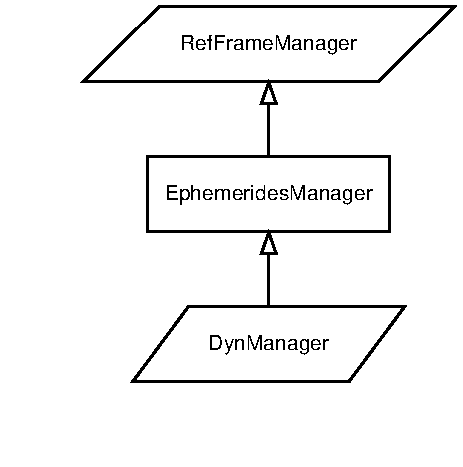
\includegraphics{ephem_manager}
\caption{Manager Classes}
\label{fig:ephem_manager_classes}
\end{figure}

\subsubsection{JPL Development Ephemeris}
The Development Ephemeris module (model subdirectory de4xx\_ephem)
defines a number of classes pertaining to reading and using a JPL
Development Ephemeris (DE) model.

These JPL ephemerides have 
been made publicly available in the form of Chebyshev polynomial coefficients.  
The DE405, DE421 and DE440 models, used by the \ModelDesc, are well accepted in 
the aerospace industry. It covers roughly 600 years from 1600 to 2170 \cite{MG} 
with DE440 covering 1550 to 2550.

These models are based on least-squares fits of observation data 
followed by a rigorous numerical integration of the equations of motion 
of the solar system bodies \cite{heafner}.
The observation data consist of optical 
transits of the Sun and planets since 1911, radar ranging to Mercury and 
Venus since 1964, tracking of deep space probes, planetary orbiters and 
landers since 1971, and lunar laser ranging since 1970 \cite{MG}.  The 
force models include point mass gravity of the Moon, planets, Sun, and 
selected asteroids; a relativistic post-Newtonian correction; luni-solar 
torques on the figure of the Earth; and Earth and Sun torques on the 
figure of the Moon \cite{MG,Seidelmann}.  Numerical integration of equations 
of motion used a variable step-size, variable order Adams method.  The 
maximum allowable integration order was 14 \cite{Seidelmann}.

Additional information regarding the Development Ephemeris models 
(and other information) can be found on the JPL Solar System 
Dynamics web page \href{http://ssd.jpl.nasa.gov}{\em http://ssd.jpl.nasa.gov}.  
The web page has an online ephemeris application tool called HORIZONS.

The implementation of the Development Ephemeris module defines several classes.\begin{description}
\item[Development Ephemeris] The class \texttt{De4xxEphemeris} is an
ephemeris model (the class derives from \texttt{EphemerisInterface})
and provides the external interface to the Development Ephemeris module.
This class contains several \texttt{EphemerisItem} objects (described above)
and a single \texttt{De4xxFile} object (described below).

\item[Ephemeris File] The class \texttt{De4xxFile} encapsulates the processes
of reading and interpreting the contents of a JPL ephemeris file. This class
contains instances of several classes and structs intended for use in this 
class only.
\begin{description}
\item[\texttt{De4xxFileHeader}] contains the header of a
Development Ephemeris file.
\item[\texttt{De4xxFileCoef}] contains the Chebyshev polynomial coefficients
that form the bulk of a Development Ephemeris file.
\item[\texttt{De4xxFileIO}] provides the library and symbol loading
mechanism to obtain data from the Development Ephemeris source data 
\item[\texttt{De4xxFileItem}] contains a description of a single item
(a planet position, barycenter position, or lunar orientation) in a
Development Ephemeris file.
\item[\texttt{De4xxFileRefTime}] converts time as represented
in JEOD to time as represented in the a Development Ephemeris file.
\item[\texttt{De4xxFileRestart}] reopens the relevant Development Ephemeris file
on restart, making a \texttt{De4xxFile} object (and by extension, the
containing \texttt{De4xxEphem} object) checkpointable and restartable.
\item[\texttt{De4xxFileSpec}] specifies the Development Ephemeris file
that is to be used in a simulation.
\item[\texttt{EphemerisDataSetMeta}] contains properties pertaining to a 
Development Ephemeris version retrieved from its shared library
\item[\texttt{EphemerisDataItemMeta}] contains properties for an ephemeris item
modeled within a DE version and retrieved from its shared library
\item[\texttt{EphemerisDataSegmentMeta}] contains properties for a portion or 
segment of a DE model usually split up by a span of 20 or 50 years retrieved
from its shared library
\end{description}

\item[Enumerations] The class \texttt{De4xxBase} encapsulates two enumerations
used in the module. One enumeration, \texttt{De4xxFileBodies}, names the
planetary items in the order implemented in a JPL ephemeris file. The
other, \texttt{De4xxEphemBodies}, names the modeled items in the order
they are implemented in the \texttt{De4xxEphemeris} class.
\end{description}

\subsubsection{Propagated Planet}
The propagated planet module (model subdirectory propagated\_planet)
provides planetary state via a DynBody object whose state can be propagated using the JEOD state integration techniques.
Scenarios in which a simulation will use a PropagatedPlanet object include:
\begin{itemize}
\item An object such as an asteroid for which an ephemeris model is not readily
available.
\item An object such as a planet that is represented in some other ephemeris
model but the simulation developer wants the planet to be propagated to
ensure that the planet and the vehicles operating in the vicinity of the
planet obey the same laws of physics.
\end{itemize}
The propagated planet module provides mechanisms that accommodate these
scenarios.
The class PropagatedPlanet defines multiple modes in which a propagated planet
planet object operates. In all modes, the model ensures consistency between
the translational states of the dynamic body's composite frame and the
planet's planet-centered frame and between the rotational states of the
dynamic body's composite frame and the planet's planet-fixed frame.


%%%%%%%%%%%%%%%%%%%%%%%%%%%%%%%%%%%%%%%%%%%%%%%%%%%%%%%%%%%%%%%%%%%%%%%%%%%%%%%%
\section{Mathematical Formulations}
\subsection{Chebyshev Approximation}
\label{sec:chebyshev_approximation}
The Development Ephemeris models released for public use contain Chebyshev
polynomial coefficients that describe the positions of the planets as
functions of time. This polynomial representation 
requires significantly fewer data points than the complete set of position
and velocity vectors for all solar system bodies at each time step 
in the numerical integration of the equations of motion. The polynomial form 
also allows users to readily interpolate between the fixed time steps of the 
ephemeris as required. 

The full time span of the DE405 ephemeris of each solar system body was 
segmented into contiguous intervals (i.e. granules) of fixed length.  
Different bodies were given different granule lengths as required to ensure 
the desired level of accuracy. Nine pairs of position and velocity values 
were selected for each granule at equally spaced times, one pair at each 
endpoint and seven pairs in between.  A constrained least-squares technique 
was used to fit Chebyshev coefficients to the position and velocity pairs such 
that the resulting Chebyshev polynomials were an exact fit at the endpoints.  
This ensured continuity between adjacent granules \cite{MG,Seidelmann}.

Chebyshev polynomials are defined as
\begin{equation}
T_n(\tau)=\cos(n\cdot \mbox{arccos } \tau)
\label{cheb_poly}
\end{equation}
where $|\tau | \le 1$.  The polynomials have the following recursive
properties:
\begin{equation}
\begin{aligned}
T_0(\tau) &= 1 \\
T_1(\tau) &= \tau \\
T_{n+1}(\tau) &= 2\tau T_n(\tau)-T_{n-1}(\tau) \mbox{   for   } n\ge 1\\
\end{aligned}
\label{cheb_recursive}
\end{equation}
A function $f(t)$ can be represented with a Chebyshev polynomial from the 
following approximation
\begin{equation}
f(t)\approx\sum^{n-1}_{i=0} a_i T_i(\tau)
\end{equation}
where $a_i$ are the coefficients determined by least-squares adjustment.

The function input time $(t)$ must fall within the interval of the 
appropriate granule of data, $t_1\le t \le t_2$.  Because the Chebyshev 
polynomials are only valid in the interval $-1\le \tau \le 1$, the reference 
time $t$ is mapped to the associated time $\tau$ in the allowable polynomial 
interval using the equation
\begin{equation}
\frac{t-t_1}{t_2-t_1}=\frac{\tau - (-1)}{1-(-1)}
\end{equation}
Solving for $\tau$ yields
\begin{equation}
\tau=2 \frac{t-t_1}{t_2-t_1}-1
\end{equation}

The time derivatives of the Chebyshev polynomials exist as analytical 
expressions.  These expressions could be used to compute velocities 
from position polynomials.  In the case of the DE405 ephemeris, 
Chebyshev polynomials were fit directly to the velocity components 
resulting from numerical integration. No differentiation is required in 
order to approximate velocity.

%%%%%%%%%%%%%%%%%%%%%%%%%%%%%%%%%%%%%%%%%%%%%%%%%%%%%%%%%%%%%%%%%%%%%%%%%%%%%%%%
\section{Interactions}
\label{sec:interactions}

\subsection{JEOD Models Used by the \ModelDesc}
The \ModelDesc uses the following JEOD models:
\begin{itemize}
\item\hypermodelref{CONTAINER}.\\
The \ModelDesc uses registry as the basis for
checkpointing the contents of the checkpointable objects at checkpoint time
and for restoring the contents of the checkpointable objects at restart time.

\item\hypermodelref{DYNBODY}.\\
The propagated planet module models planets as dynamic bodies
so that they can be propagated if desired.

\item\hypermodelref{MATH}.\\
The \texttt{EphemerisZXZOrientation} class uses the vector capabilities
defined in the \MATH.

\item\hypermodelref{MEMORY}.\\
As do almost all other models,
the \ModelDesc uses the \MESSAGE\ to manage dynamically-allocated memory.

\item\hypermodelref{MESSAGE}.\\
As do almost all other models,
the \ModelDesc uses the \MESSAGE\ to generate messages.

\item\hypermodelref{NAMEDITEM}.\\
Various modules use the \NAMEDITEM\ to construct and validate names.

\item\hypermodelref{PLANET}.\\
Ephemerides that pertain to planetary bodies (which includes the Sun) are
stored in one of the reference frames contained in a
\texttt{BasicPlanet} object.

\item\hypermodelref{QUATERNION}.\\
The \texttt{EphemerisZXZOrientation} class uses quaternions to
propagate the rotational state between updates.

\item\hypermodelref{REFFRAMES}.\\
External users of the \ModelDesc access ephemerides
via the reference frames in which those ephemerides are stored.

\item\hypermodelref{SIMINTERFACE}.\\
As do almost all other models,
the \ModelDesc uses the \SIMINTERFACE\ to make model data and functions
visible to the simulation engine.

\item\hypermodelref{TIME}.\\
The DE4xx ephemeris and propagated planet modules use the the \TIME\ to
timestamp reference frames.
The DE4xx ephemeris module also uses the \TIME\ to obtain the current
Terrestrial Time. The JPL ephemerides are Chebyshev polynomials in time.
\end{itemize}

\subsection{JEOD Models That Use the \ModelDesc}
\begin{itemize}
\item Multiple models.\\
The \hypermodelref{BODYACTION}, \hypermodelref{DYNBODY}, and
\hypermodelref{GRAVITY} use pointers and references to
instances of the \texttt{EphemerisRefFrame} class and
use the \texttt{EphemeridesManager} to find reference frames
and planets.

\item\hypermodelref{DYNMANAGER}.\\
The \texttt{DynManager} class defined in the \DYNMANAGER\ derives from the
\texttt{EphemeridesManager} class.
The \texttt{DynamicsIntegrationGroup} class uses the
\texttt{EphemeridesManager} (via the \texttt{DynManager})
to update ephemerides.

\item\hypermodelref{PLANET}.\\
The \texttt{BasePlanet} class defined in the \PLANET\ contains
instances of the \texttt{EphemerisRefFrame} class, one for the
planet-centered inertial frame and the other for the planet-centered,
planet-fixed frame. \texttt{BasePlanet} instances register themselves
and the frames they contain with the \texttt{EphemeridesManager}.

\item\hypermodelref{RNP}.\\
The \texttt{PlanetOrientation} class defined in the \RNP\ derives from
the \texttt{EphemerisInterface} class and contains an
\texttt{EphemerisOrientation} object. \texttt{PlanetOrientation}
instances register themselves as ephemeris models with
the \texttt{EphemeridesManager}.
\end{itemize}


%%%%%%%%%%%%%%%%%%%%%%%%%%%%%%%%%%%%%%%%%%%%%%%%%%%%%%%%%%%%%%%%%%%%%%%%%%%%%%%%
\section{Detailed Design}
Details of the design of the JEOD \ModelDesc can be found in
\hyperref{file:refman.pdf}{}{}
{JEOD Ephemerides Model Reference Manual}~\cite{ephemerides_refman}.

\clearpage
\boilerplateinventory
